%%% template.tex
%%%
%%% This LaTeX source document can be used as the basis for your technical
%%% paper or abstract. Intentionally stripped of annotation, the parameters
%%% and commands should be adjusted for your particular paper - title, 
%%% author, article DOI, etc.
%%% The accompanying ``template.annotated.tex'' provides copious annotation
%%% for the commands and parameters found in the source document. (The code
%%% is identical in ``template.tex'' and ``template.annotated.tex.'')

\documentclass[]{acmsiggraph}
\usepackage{algorithm}
\usepackage[noend]{algpseudocode}
\TOGonlineid{45678}
\TOGvolume{0}
\TOGnumber{0}
\TOGarticleDOI{0}
\TOGprojectURL{}
\TOGvideoURL{}
\TOGdataURL{}
\TOGcodeURL{}
\usepackage{color}
%\definecolor{red}{rgb}{0.9, 0.17, 0.31}
\usepackage{multirow}
\usepackage{subfig}
\usepackage{xcolor}
\usepackage{lipsum}
\usepackage{listings}
\usepackage{graphicx}
\usepackage{glsllst} % My own package providing markup listing for glsl
\usepackage{rmlst}   % My own package providing markup listing for renderman
\usepackage{amsmath}
\usepackage{hyperref}

\lstset{
	backgroundcolor=\color[rgb]{0.95, 0.95, 0.95},
	tabsize=3,
	%rulecolor=,
	basicstyle=\footnotesize\ttfamily,
	upquote=true,
	aboveskip={1.5\baselineskip},
	columns=fixed,
	showstringspaces=false,
	extendedchars=true,
	breaklines=true,
	prebreak = \raisebox{0ex}[0ex][0ex]{\ensuremath{\hookleftarrow}},
	frame=none,
	aboveskip=15pt,
	belowskip=8pt,
	captionpos=t,
	showtabs=false,
	showspaces=false,
	showstringspaces=false,
	identifierstyle=\ttfamily,
	%keywordstyle=\color{red}\bfseries,
	%keywordstyle=[1]\bfseries\color{syntaxBlue},
	%keywordstyle=[2]\bfseries\color{syntaxRed},
	%keywordstyle=[3]\color{blue}\bfseries,
	%keywordstyle=[4]\bfseries\color{syntaxBlue},
	commentstyle=\color[rgb]{0.082,0.639,0.082},
	keywordstyle=[1]\bfseries\color[rgb]{0,0,0.75},
	keywordstyle=[2]\bfseries\color[rgb]{0.5,0.0,0.0},
	keywordstyle=[3]\bfseries\color[rgb]{0.127,0.427,0.514},
	keywordstyle=[4]\bfseries\color[rgb]{0.4,0.4,0.4},
	stringstyle=\color[rgb]{0.639,0.082,0.082},
}

\title{Principles of Rendering: Offline Rendering}

\author{Callum Glover\thanks{e-mail:s4907224@bournemouth.ac.uk}\\National Centre for Computer Animation}
\pdfauthor{Callum Glover}

\keywords{rendering}

\begin{document}

%% \teaser{
%%   \includegraphics[height=1.5in]{images/sampleteaser}
%%   \caption{Spring Training 2009, Peoria, AZ.}
%% }

\maketitle


\begin{abstract}
Abstract text goes here.
\end{abstract}
%\keywordlist
%\TOGlinkslist

\section{Introduction} \label{sec:introduction}
Introduciton goes here.

\begin{figure}[htbp]\centering
 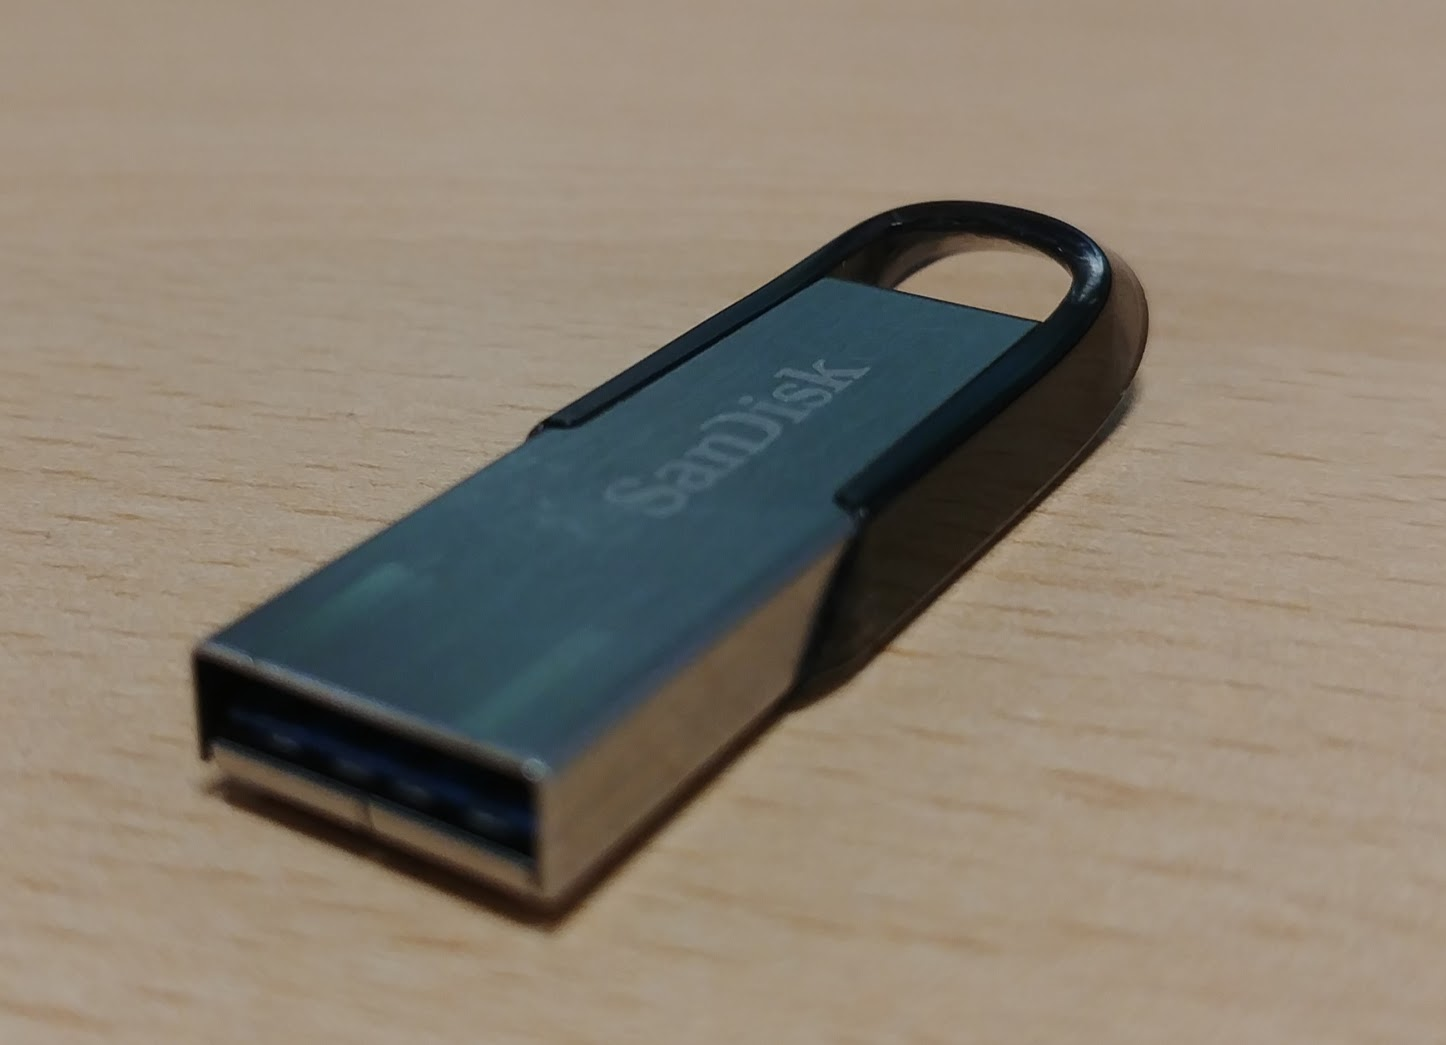
\includegraphics[width=0.75\linewidth]{images/photoref.jpg}
 \caption{\label{fig:reference}The original reference image.}
\end{figure}

\begin{figure}[htbp]\centering
 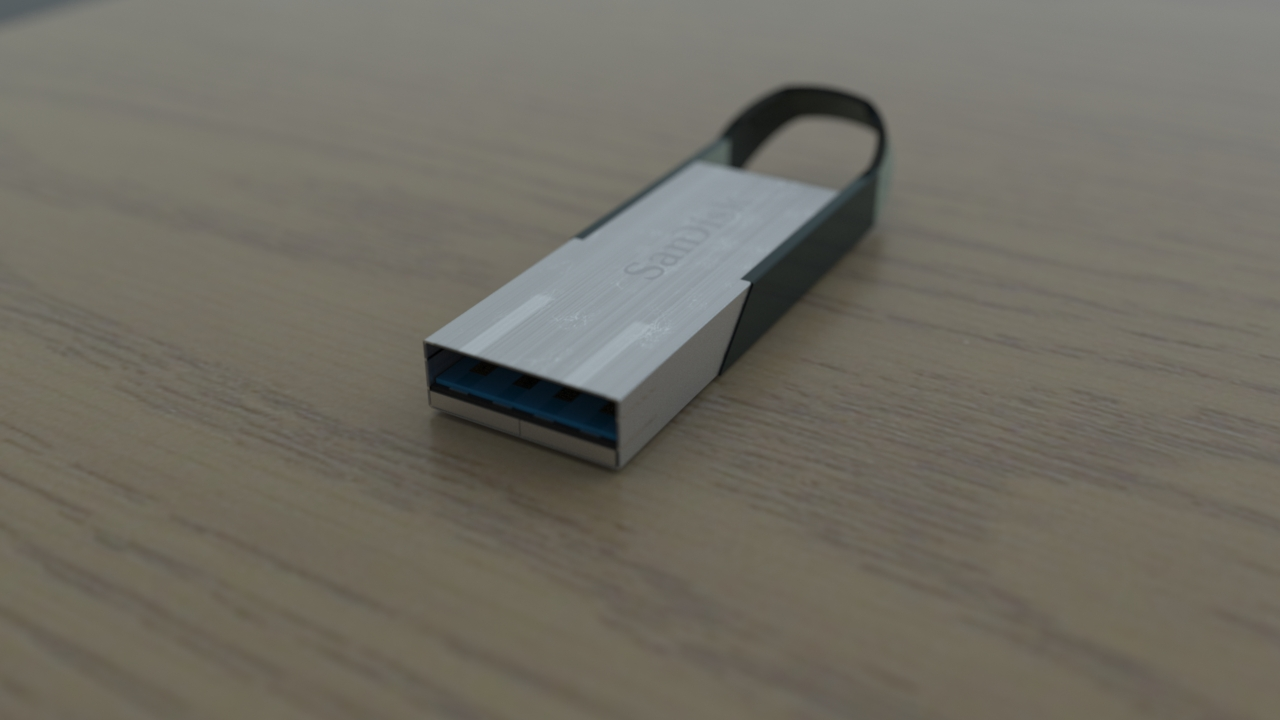
\includegraphics[width=0.75\linewidth]{images/sd.jpg}
 \caption{\label{fig:CG}The final rendered CG image.}
\end{figure}

Breaking down the properties seen in~\ref{fig:reference}:
\begin{enumerate}
 \item A brushed metal like appearance, resulting in narrow changing bands of roughness, having an effect on the specular highlights.
 \item Small worn patches where the USB is plugged in frequently.
 \item A glossier plastic back loop.
 \item Non metallic, rough decal.
 \item Soft shadowing.
 \item Small, narrow depth of field.
\end{enumerate}


\section{Method Overview} \label{sec:overview}
Text goes here. Eq reference like this Equation~\ref{eq:kajiya}.
\begin{multline}\label{eq:kajiya}
L_o \left( \mathbf{x},\omega_o,\lambda,t \right) = L_e\left(\mathbf{x},\omega_o,\lambda,t \right) + \\
   \int_\Omega f_r \left(\mathbf{x},\omega_i,\omega_o,\lambda,t\right) L_i\left(\mathbf{x},\omega_i,\lambda,t\right) \left(\omega_i \cdot \mathbf{n}\right) d\omega_i
\end{multline}
Text goes here. Alg reference like this Algorithm~\ref{alg:euclid}. 
\begin{algorithm}
\caption{Euclid’s algorithm}\label{alg:euclid}
\begin{algorithmic}[1]
\Procedure{Euclid}{$a,b$}\Comment{The g.c.d. of a and b}
\State $r\gets a\bmod b$
\While{$r\not=0$}\Comment{We have the answer if r is 0}
\State $a\gets b$
\State $b\gets r$
\State $r\gets a\bmod b$
\EndWhile\label{euclidendwhile}
\State \textbf{return} $b$\Comment{The gcd is b}
\EndProcedure
\end{algorithmic}
\end{algorithm}
You can footnote like this \footnote{See \url{https://en.wikipedia.org/wiki/Data_flow_diagram}.} then more text goes here.

You can reference appendices like this : Appendices~\ref{app:renderman} and~\ref{app:glsl}.

\section{Results} \label{sec:results}
And sections like this : Section~\ref{sec:overview} and other figures like this : (see Figure~\ref{fig:comparison} for an example). and more text can follow.

\begin{figure}[htbp]
  \centering
 \subfloat[Diff+Spec]{
\includegraphics[width=0.45\linewidth]{images/image1.jpg}}
 \hfill
 \subfloat[Diff+Spec+Ambient]{
\includegraphics[width=0.45\linewidth]{images/image2.jpg}}
 \caption{\label{fig:comparison}More image caption These were appropriated from \protect\cite{renderman16}.}
\end{figure}

Text and shizzle.

\bibliographystyle{acmsiggraph}
\bibliography{references}

\newpage
\appendix
\section{Renderman Shader Example}\label{app:renderman}
This is how to reference code.
\begin{lstlisting}[language=rendermansl, label={lst:renderman}, caption={Renderman example lifted from \protect\cite{renderman16}.}]
surface basicSpecular(
    color myOpacity = 1; 
    float roughness = 0.1;
)
{
        color myColor = (1.0, 0.0, 0.0);
        normal Nn = normalize(N);
        //Specular stuff
        vector V = normalize(-I);
        
        Ci = myColor * myOpacity * diffuse(Nn) + specular(Nn, V, roughness);
        Oi = myOpacity;
} 
\end{lstlisting}


\section{GLSL Shader Example}\label{app:glsl}
This is how to reference code.

\begin{lstlisting}[language=GLSL, label={lst:glsl}, caption={A simple textured shader.}]
// The texture coordinates
smooth in vec2 o_TexCoord;

// This is passed on from the vertex shader
in vec3 LightIntensity;

// The texture to be mapped
uniform sampler2D u_Texture;

// This is no longer a built-in variable
out vec4 o_FragColor;

void main() {
    // Set the output color of our current pixel
    o_FragColor = vec4(LightIntensity,1.0) * texture(u_Texture, o_TexCoord);
}
\end{lstlisting}


\end{document}

